\documentclass[a4paper,10pt]{article}
\usepackage[utf8]{inputenc}

% ----  Useful packages % ---- 
\usepackage{amsmath}
\usepackage{graphicx}
\usepackage{amsfonts}
\usepackage{amsthm}
\usepackage{amssymb}
\usepackage{makecell}
\usepackage{array}
\usepackage{booktabs}
\usepackage{multirow}
% ----  Useful packages % ---- 

\usepackage{wrapfig}
\usepackage{caption}
\usepackage{subcaption}
\usepackage{hyperref}
\hypersetup{
    colorlinks,
    citecolor=black,
    filecolor=black,
    linkcolor=black,
    urlcolor=black
}

\graphicspath{ {./images/} }

% ---- Set page size and margins replace ------
\usepackage[letterpaper,top=2cm,bottom=2cm,left=3cm,right=3cm,marginparwidth=1.75cm]{geometry}
% ---- Set page size and margins replace ------

% ------- NOTA ------
\theoremstyle{remark}
\newtheorem{note}{Note}[subsubsection]
% ------- NOTA ------

% ------- OSSERVAZIONE ------
\theoremstyle{definition}
\newtheorem{observation}{Osservazione}[subsection]
% ------- OSSERVAZIONE ------

% ------- DEFINIZIONE ------
\theoremstyle{plain}
\newtheorem{definition}{Definition}[subsection]
% ------- DEFINIZIONE ------

% ------- ESEMPIO ------
\theoremstyle{definition}
\newtheorem{example}{Esempio}[subsection]
% ------- ESEMPIO ------

% ------- DIMOSTRAZIONE ------
\theoremstyle{definition}
\newtheorem{demostration}{Dimostrazione}[subsection]
% ------- DIMOSTRAZIONE ------

% ------- TEOREMA ------
\theoremstyle{definition}
\newtheorem{theorem}{Teorema}[subsection]
% ------- TEOREMA ------

% ------- COROLLARIO ------
\theoremstyle{plain}
\newtheorem{corollaries}{Corollario}[theorem]
% ------- COROLLARIO ------

% ------- PROPOSIZIONE ------
\theoremstyle{plain}
\newtheorem{proposition}{Proposizione}[subsection]
% ------- PROPOSIZIONE ------

% ---- Footer and header ---- 
\usepackage{fancyhdr}
\pagestyle{fancy}
\fancyhf{}
\fancyhead[LE,RO]{A.A 2022-2023}
\fancyhead[RE,LO]{Systems Software}
\fancyfoot[RE,LO]{\rightmark}
\fancyfoot[LE,RO]{\thepage}

\renewcommand{\headrulewidth}{.5pt}
\renewcommand{\footrulewidth}{.5pt}
% ---- Footer and header ---- 

% ----  Language setting ---- 
\usepackage[italian, english]{babel}
% ----  Language setting ---- 

\usepackage{listings}
\usepackage{color}

\definecolor{dkgreen}{rgb}{0,0.6,0}
\definecolor{gray}{rgb}{0.5,0.5,0.5}
\definecolor{mauve}{rgb}{0.58,0,0.82}

\lstset{frame=tb,
  language=C,
  aboveskip=3mm,
  belowskip=3mm,
  showstringspaces=false,
  columns=flexible,
  basicstyle={\small\ttfamily},
  numbers=none,
  numberstyle=\tiny\color{gray},
  keywordstyle=\color{blue},
  commentstyle=\color{dkgreen},
  stringstyle=\color{mauve},
  breaklines=true,
  breakatwhitespace=true,
  tabsize=3
}

\title{\textbf{Systems Software}}
\author{Autor: Ghirardini Filippo}
\date{Winter Semester 2024-2025}

\begin{document}
\begin{titlepage} %crea l'enviroment
	\begin{figure}[t] %inserisce le figure
		\centering
\includegraphics[width=0.98\textwidth]{marchio_unipi_pant541.png}
	\end{figure}
	\vspace{20mm}
	
	\begin{Large}
		\begin{center}
			\textbf{Dipartimento di Informatica\\ Corso di Laurea Triennale in Informatica\\}
			\vspace{20mm}
			{\LARGE{Corso a Libera Scelta - 6 CFU}}\\
			\vspace{10mm}
			{\huge{\bf Computer Graphics}}\\
		\end{center}
	\end{Large}
	
	
	\vspace{36mm}
	%minipage divide la pagina in due sezioni settabili
	\begin{minipage}[t]{0.47\textwidth}
		{\large{\bf Professore:}\\ \large{Prof. }}
	\end{minipage}
	\hfill
	\begin{minipage}[t]{0.47\textwidth}\raggedleft
		{\large{\bf Autore:}\\ \large{Filippo Ghirardini}}
	\end{minipage}
	
	\vspace{25mm}
	
	\hrulefill
	
	\vspace{5mm}
	
	\centering{\large{\bf Anno Accademico 2023/2024 }}
	
\end{titlepage}

\tableofcontents
\newpage
\maketitle
\begin{center}
    \vspace{-20pt}
    \rule{11cm}{.1pt} 
\end{center}
\newpage
\section{Punto materiale}
Oggetto caratterizzato da una massa [kg] e da un vettore posizione [m] nello spazio 3D.
Dimensioni trascurabili, forma irrilevante rispetto ai fenomeni di interesse.
Vettore posizione come funzione del tempo t[s].
\begin{example}
    Una molecola di ossigeno se sono interessato all'aereodinamica di una vettua. 
    Un satellite attorno alla terra se ignoro le forze di marea.
\end{example}
\hspace{-15pt}\textbf{Un vettore posizione} è una funzione del tempo $t[s]$.
$$\vec{r(t)} = (x(t), y(t), z(t)) = x(t)\hat{x} + y(t)\hat{z} + z(t)\hat{z}$$
\begin{observation}
    I versori cartesiani sono costanti
\end{observation}

\begin{definition}[Legge oraria]
    Si definisce come legge oraria la funzione $t \mapsto \vec{r}(t)$.
\end{definition}

\begin{definition}[Traiettoria]
    Il luogo geometrico di punti visitati dal punto materiale.
    $$\{\vec{r}(t)\:\: per \: t \in \mathbb{R}\}$$
\end{definition}

\begin{example}
    $\vec{r}(t) = (v_0t, y_0, 0)$ e $v_0 = 3m/s, y_o = 5m$ 
    \begin{figure}[h!]
        \centering
        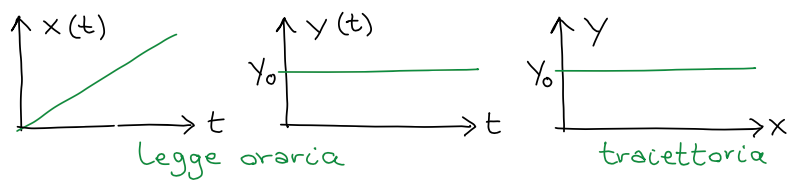
\includegraphics[width=0.8\textwidth]{images/ess-traiettoria.png}
    \end{figure}
\end{example}

\begin{definition}
    La \textbf{velocità istantanea} è la derivata della posizione rispetto al tempo.
    $$v = \lim_{\Delta t \to 0}\frac{\Delta s}{\Delta t} = \frac{ds}{dt}$$
\end{definition}

\begin{definition}
    La \textbf{velocità media} è definita come il rapporto tra lo spostamento e l'intervallo di tempo necessario per effettuarlo.
    $$v_m = \frac{\Delta s}{\Delta t}$$
\end{definition}
\hspace{-15pt}In parole povere è una grandezza che ci dice con quale rapidità cambia la posizione di un punto rispetto al tempo nell'instante $t$.
\subsection*{Vettore velocità}
Derivata rispetto al tempo del vettore posizione e si indica come 
$\frac{d\vec{r}(t)}{dt}\text{ oppure }\dot{\vec{r}}(t)[m/s]$
\begin{equation}
    \begin{split}
    \dot{\vec{r}}(t) & = (\dot{x}(t), \dot{y}(t), \dot{z}(t)) \\
     & = \frac{d}{dt}[x(t)\hat{x} + y(t)\hat{y} + z(t)\hat{z}] \\
     & = \dot{x}(t)\hat{x} + \dot{y}(t)\hat{y} + \dot{z}(t)\hat{z}
    \end{split}
\end{equation}
Per ricavare la forma esplicita uso le proprietà delle derivate (\textbf{linearità}, \textbf{Leibnitz})
\begin{example}
    $\vec{r}(t) = (v_0t, y_0, 0) = v_0t\hat{x} + y_0\hat{y}$ \:\:\:abbiamo che \:\:\:
    $\dot{\vec{r}}(t) = (v_0, 0, 0) = v_0 \hat{x}$
\end{example}
\hspace{-15pt}Velocità e spazio percorso ("integrale di linea").\\
\begin{wrapfigure}[3]{l}{5cm}
    \centering
    \includegraphics[width=5cm]{images/vettore-velocità.png}
\end{wrapfigure}
\begin{align*}
    L & = ||\vec{r}(t_1) - \vec{r}(t_0)|| + ||\vec{r}(t_2) - \vec{r}(t_1)|| + ||\vec{r}(t_3) - \vec{r}(t_2)|| + \dots \\
    & = \sum_i ||\vec{r}(t_{i+1} - \vec{r}(t_i)|| \:\: per\:\: |t_{i+1} - t_i| \text{"piccolo"} \\
    & = \sum_i ||\frac{\vec{r}(t_{i+1}) - \vec{r}(t_i)}{t_{i+1} - t_i}|| (t_{i+1} - t_i) = \int_{t_{in}}^{t_{f_{in}}}||\dot{\vec{r}}(t)||\\
\end{align*}
\begin{example}
    $\vec{r}(t) = (v_0t, y_0)\:\:\: \dot{\vec{r}}(t) = (v_0, 0)$\hspace{15pt}
    $||\dot{\vec{r}}(t)|| = \sqrt{v_0^2 + 0^2} = |v_0|$ \:\:\: $L = |v_0| \cdot (t_{f_{in}} - t_{in})$\\
    Il vettore è costante quindi facendo la derivata torna zero. Con la velocità si calcolo lo spazio percorso ("integrale di linea").
    La differenza fra le posizioni e la differenza dei tempi è il rapporto incrementale in caso gli intervalli siano sufficentemente
    piccoli, da qui si ottiene l'integrale.
\end{example}

\subsection{Vettore accelerazione}
Derivata rispetto al tempo del vettore velocità e si indica con $\frac{d^2\vec{r}(t)}{dt} \text{ oppure } \ddot{\vec{r}}(t) [m/s^2]$
\begin{equation}
    \ddot{\vec{r}}(t) = (\ddot{x}(t), \ddot{y}(t), \ddot{z}(t))\:\: = \:\: \ddot{x}(t)\hat{x} + \ddot{y}(t)\hat{y} + \ddot{z}(t)\hat{z}
\end{equation}
\begin{example}
    $\vec{r}(t)= (\frac{1}{2}a_0t^2, v_0t, 0)$ \hspace{10pt} $\dot{\vec{r}}(t) = (a_0t, v_0, 0)$ \hspace{10pt} $\dot{\vec{r}}(t) = (a_0, 0, 0)$
\end{example}
\hspace{-15pt}Serve perché l'equazione "del moto" di Newton che determinata la legge oraria è formulata in termini di accelerazione.

\subsection{Vettore quantità di moto}
Il prodotto di massa [kg] e velocità [m/s]
$$\vec{p}(t) = m \cdot \dot{\vec{r}}(t) = (m\dot{x}(t), m\dot{y}(t), m\dot{x}(t)) = m\dot{\vec{x}}(t)x + m\dot{\vec{y}}(t)y + m \dot{\vec{z}}(t)z$$
\begin{example}
    Prendiamo un punto di massa 2kg e velocità 3m/s lungo $\hat{x}$.\\
    $p_x(t) = 2 \cdot 3 kg\cdot m/s = 6 kg \cdot m/s$ \hspace{15pt} $p_y(t) = p_z(t) = 0$.
\end{example}
\hspace{-15pt}Serve per generalizzare l'equazione di Newton e per trattare sistemi di piu punti materiali.

\subsection{Vettore momento angolare rispetto a un polo P}
$$\vec{L}_p(t) = m(\vec{r}(t) - \vec{r}_p) \times \dot{\vec{r}}(t)$$
Dove $\vec{r}_p$ è il vettore posizione di p, mentre $\dot{\vec{r}}(t)$ è il prodotto vettoriale.
\begin{example}
    $\vec{r}_p = (l_0, 0, 0)$ \hspace{15pt} $\vec{r}(t) = (v_0t, y_0, 0)$\\
    $\vec{L}_p = m[(v_0t - l_0)\hat{x} + y_0\hat{y}] \times (v_0\hat{x}) \:\: = \:\: m(v_0t - l_0)v_0 \hat{x} \times \hat{x} + my_0v_0\hat{y}\times \hat{x} 
    \:\: = \:\: my_0v_0(-\hat{z}) = (0,0, -my_0v_0)$\\
    Ricorda che $\hat{x} \times \hat{x} = 0$ e $\hat{y} \times \hat{x} = -\hat{z}$
\end{example}
\hspace{-15pt}Il momento angolare dice quanta inerzia ha un oggetto in una rotazione (descrizione sommaria).\\
Il polo P è parte della definizione. È una scelta! Il risultato dipende dal polo.
Serve per formulare l'equazione del moto di sistemi di punti materiali e corpi rigidi.

\subsection{Coordinate polari}
Un metodo per rapprensentare delle cordinate x, y andando a misurare prima la distanza dall'origine e poi si va a vedere
quanto vale l'angolo fra questo segmento dall'asse x, utilizzando seno e coseno.
\begin{wrapfigure}[7]{l}{2cm}
    \centering
    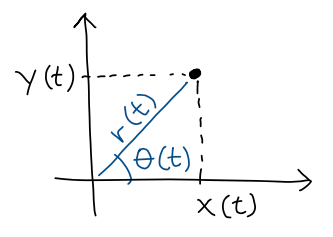
\includegraphics[width=5.5cm]{images/coordinate-polari.png}
\end{wrapfigure}
\begin{align*}
    \begin{cases}
        x(t) = r(t) \cdot \cos(\Theta(t))\\
        y(t) = r(t) \cdot \sin(\Theta(t)) 
    \end{cases}
\end{align*}
\begin{align*}
    \begin{cases}
        r(t) = \sqrt{x(t)^2 + y(t)^2} \geq 0\\
        tg(\Theta(t)) = y(t) / x(t) 
    \end{cases}
\end{align*}
\\
\begin{example} Esempi di rappresentazione di coordinate in coordinate polari.\\
    $x = 0, y = l_0 > 0 \:\: \Rightarrow \:\: r = l_0, \Theta = \pi/2$\\
    $x = 0, y = -l_0 < 0 \:\: \Rightarrow \:\: r = l_0, \Theta = -\pi/2$\\
    $x = l_0, y = l_0 > 0 \:\: \Rightarrow \:\: r = \sqrt{2}l_0, \Theta = \pi/4$\\
\end{example}

\subsection{Versori polari (2D)}
Definisco un versore $\hat{r}(t)$ che punta verso il punto materiale e un versore $\hat{\Theta}(t)$ ortogonale.
Si esprime facilmente in coordinte polari.
$$\vec{r}(t) = (x(t), y(t)) = (r(t)\cos \Theta(t), r(t)\sin\Theta(t)) \:\: = \:\: r(t)(\cos\Theta(t)\hat{x} + \sin\Theta(t)\hat{y})$$
Ma $||\vec{r}(t)|| = |r(t)| = r(t)$ allora definisco $\hat{r}(t) = \vec{r}(t)/ ||\vec{r}(t)|| = \cos \Theta(t)\hat{x} + \sin\Theta(t)\hat{y}$\\\\
Trovo facilmente che un versore ortogonale è:
$$\hat{\Theta(t)} = -\sin\Theta(t)\hat{x} + \cos\Theta(t)\hat{y} \:\:\:\text{infatti} \:\:\: \hat{r}\cdot \hat{\Theta} = c \cdot (-s) + s \cdot c = 0$$
\begin{wrapfigure}[7]{r}{6cm}
    \centering
    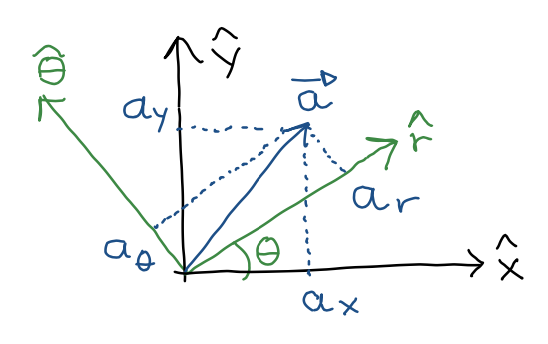
\includegraphics[width=5.5cm]{images/trasformazioni-inverse.png}
\end{wrapfigure}
\begin{note}
    Non c'è legame fra $\Theta$ e $\hat{\Theta}$ è solo una convenzione.
\end{note}
\hspace{-15pt}Le trasformazioni inverse invece si fanno come segue (verifico per sostituzione):
$$\hat{y} = \cos\Theta(t)\hat{r} - \sin\Theta(t)\hat{\Theta} \hspace{20pt} \hat{y} = \sin\Theta(t)\hat{r} + \cos\Theta(t)\hat{\Theta}$$
Possono quindi scrivere ogni vettore nella forma $\vec{a} = a_r\hat{r} + a_{\Theta}\hat{\Theta}$ con le componenti polari $a_r, a_{\Theta}$.
Per evitare ambiguità non scriviamo $(a_r, a_{\Theta})$ e riserviamo la notazione alle componenti cartesiane.\\\\
A differenza dei versori cartesiani quelli polari dipendono dal tempo per costruzioni.
$$\dot{\hat{r}}(t) = \frac{d}{dt}[\cos\Theta(t) \hat{x} + \sin\Theta(t)\hat{y}] \:\: = \:\: -\sin\Theta(t) \cdot \dot{\Theta}(t)\hat{x} + \cos\Theta(t) \cdot \dot{\Theta}(t)\hat{y}$$
Dove $\cos\Theta(t) \cdot \dot{\Theta}(t)$ si applica la derivata della somma, Leibnitz, funzione composta.
$$= \dot{\Theta}(t)\cdot \hat{\Theta}(t) \:\:\:\:(\text{confronto l'espressione di} \hat{\Theta}(t))$$
Similmente $\dot{\hat{\Theta}}(t)= - \dot{\Theta}\hat{r}(t)$.


\subsection*{Vettori posizione, velocità, accelerazione}
$$\vec{r}(t) = r(t)\hat{r}(t)$$
Dove abbiamo che $\vec{r}(t)$ è il vettore, $r(t)$ è una coordinata polare, $\hat{t}(t)$ è il versore polare.
$$\dot{\vec{r}}(r) = \dot{r}(t)\hat{r}(t) + r(t)\dot{\Theta}(t)\hat{\Theta}(t)$$
Dove la parte $\dot{\vec{r}}(r)$ è la velocità radiale.
$$\ddot{\vec{r}}(t) = [\ddot{r}(t) - r(t)\dot{\Theta}(t)^2] \hat{r} + [r(t) \ddot{\Theta}(t) + 2\dot{r}(t)\dot{\Theta}(t)]\hat{\Theta}$$
Nel quale abbiamo che la parte $r(t)\dot{\Theta}(t)^2$ si chiama \textbf{velocità centripeta}, mentre $2\dot{r}(t)\dot{\Theta}(t)$ si dice \textbf{accelerazione di Coriolis}.


\newpage
\section{Architecture}
A general system consists of  \textbf{elements} and \textbf{relationships} between them. The elements are the functional units with interaction of different kinds in between (e.g. data flow, request flow, call, etc.).\\\\
In an \textbf{operating system} the elements are the \textbf{processes} and they interact with each other.. Since they are not hardware native we need something that provides them and also the interactions: the \textbf{kernel.}. Therefore, we'll have two areas:
\begin{itemize}
	\item \textit{Process area}: where the OS functionalities are located
	\item \textit{Kernel area}: provides the fundamental infrastructure for the processes
\end{itemize}

\begin{center}
	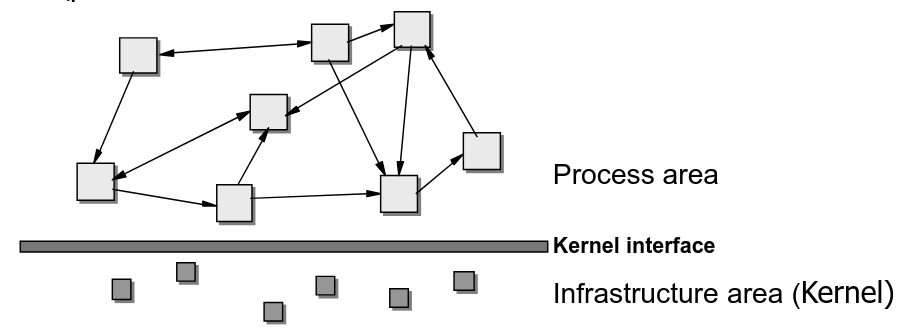
\includegraphics[scale=0.3]{kernelarea.png}
\end{center}

\subsection{Process area}
In more details, the process area is divided like this:
\begin{center}
	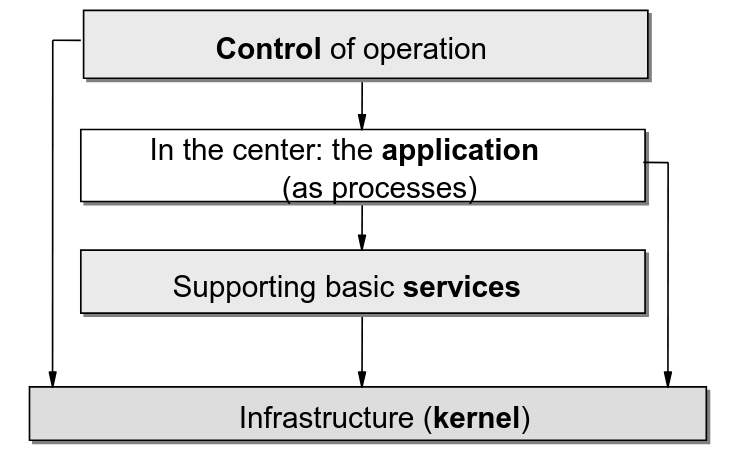
\includegraphics[scale=0.3]{processarea.png}
\end{center}
\subsubsection{Services}
In particular, services deal with \textbf{resources} needed by applications, since handling them directly is very tedious.
\begin{center}
	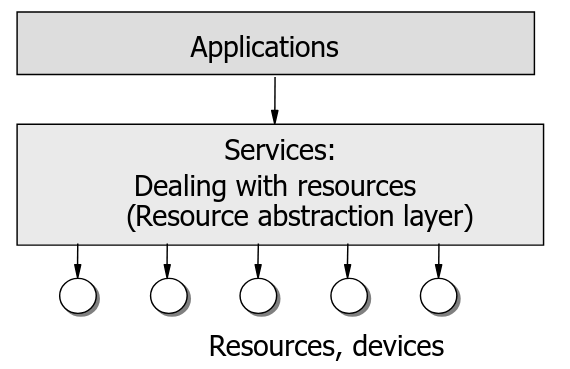
\includegraphics[scale=0.3]{services.png}
\end{center}
Therefore, we need to make a distinction between resources:
\begin{itemize}
	\item \textbf{Logical}: resources for made organizational reasons  by real ones (e.g. files)
	\item \textbf{Physical}: real existent (e.g. mouse, keyboard)
\end{itemize}
The main two aspects of dealing with resources are:
\begin{itemize}
	\item \textbf{Management}: in case of competition, deciding who should get the resource and when
	\begin{center}
		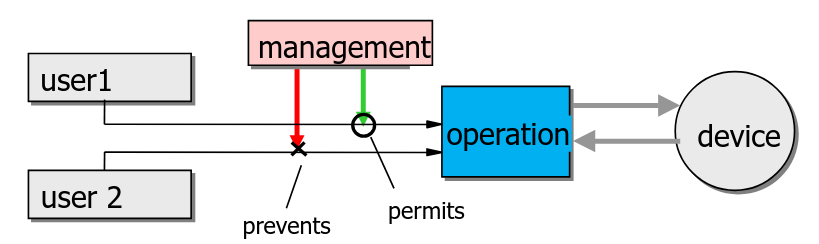
\includegraphics[scale=0.3]{management.png}
	\end{center}
	\item \textbf{Operation}: real usage (e.g. data transport) with \textbf{read} and \textbf{write} operations
	\begin{center}
		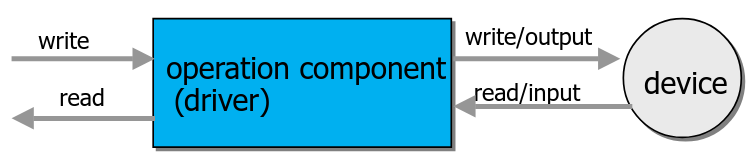
\includegraphics[scale=0.3]{operation.png}
	\end{center}
\end{itemize}
In the end we have both the \textit{management} and the \textit{operation} for the \textit{logical} resources and for the \textit{real} ones.

\subsubsection{Control}
We distinguish two interfaces:
\begin{itemize}
	\item \textbf{Control} interface: handles the interactions between the user and the machine (OS commands and UI)
	\item \textbf{Procedural} interface: has the possibility to make complex requests to the OS, also with programming language notation
\end{itemize}

\subsubsection{Overview}
\begin{center}
	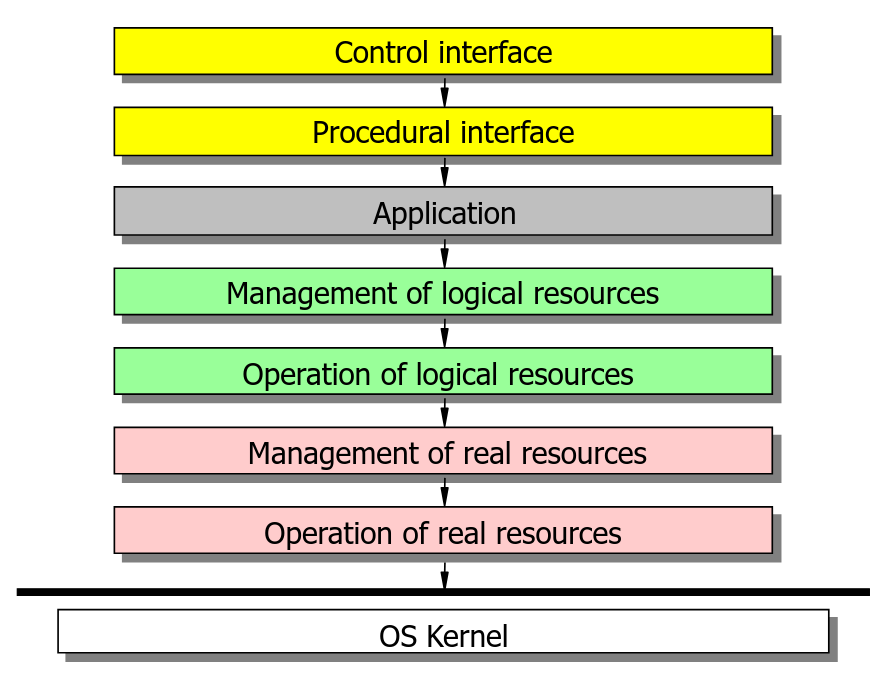
\includegraphics[scale=0.4]{overview.png}
\end{center}

\begin{note}
	Each layer may be \textbf{partitioned} and upward calls are allowed as long as there are no cycles.
\end{note}

\subsection{Kernel area}
In details, the kernel area is divided like this:
\begin{center}
	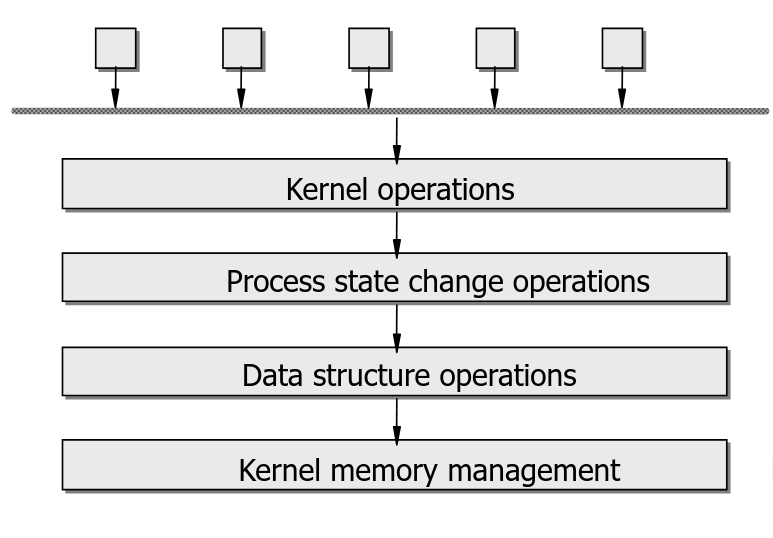
\includegraphics[scale=0.3]{kernelareaover.png}
\end{center}
There are two ways of realizing a kernel:
\begin{itemize}
	\item \textbf{Scattered} across programs: kernel operations resides in different program address spaces
	\item \textbf{Compact}: there is the kernel address space which contains its own procedures
\end{itemize}

\subsubsection{Size}
Depending on what functionalities you add in the kernel, you may end up with different kernel sizes. The bare minimum is the one described above (process management and communication) and it's called \textbf{microkernel}.

\subsubsection{Monolithical}
Another approach is the \textbf{monolithical system}, where there is no strict separation between applications and OS. It's appropriate for small OS.
\begin{center}
	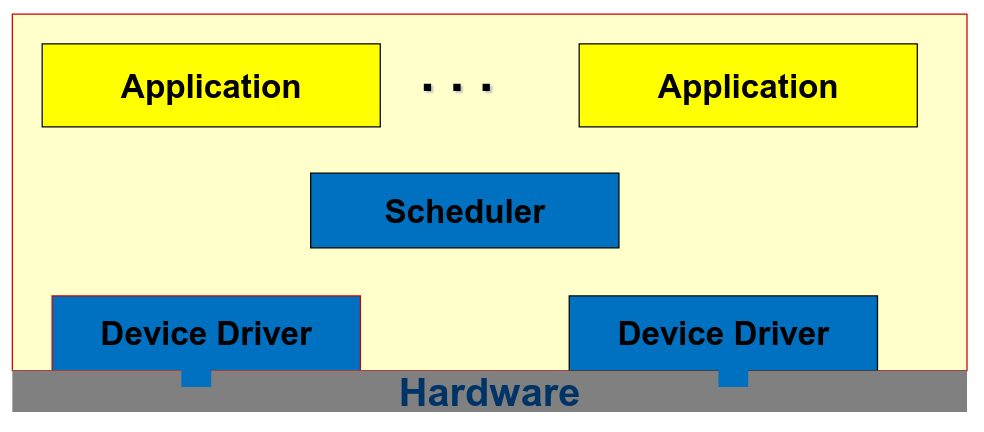
\includegraphics[scale=0.3]{monolit.png}
\end{center}
On the other hand, \textbf{monolithical OS-kernels} have a separation between applications and OS for \textbf{protection} reasons but no separations among OS components.
\begin{center}
	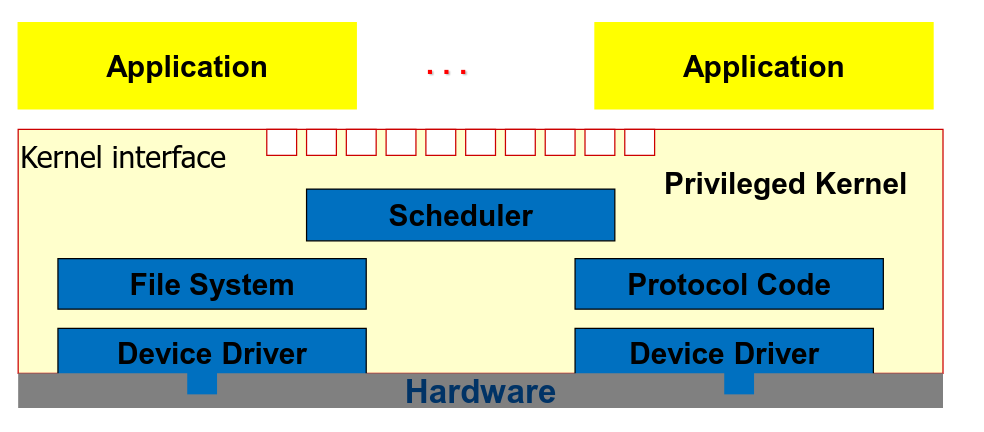
\includegraphics[scale=0.3]{monoker.png}
\end{center}

\subsubsection{Microkernel}
As stated before, a microkernel contains only process management (initializing and dispatching) and Inter Process Communication.
\begin{center}
	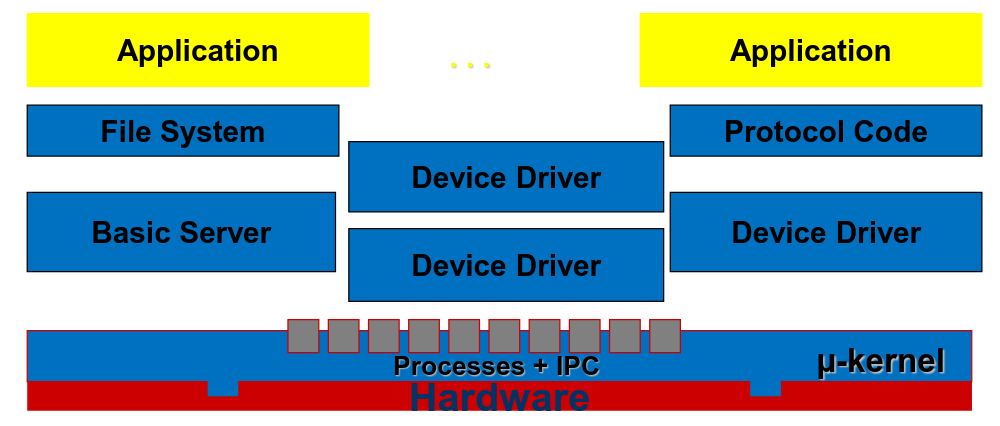
\includegraphics[scale=0.3]{microker.png}
\end{center}
The \textbf{advantages} are:
\begin{itemize}
	\item Supports \textbf{modular} structure
	\item Since the services are outside of the kernel, there is more \textbf{stability} and \textbf{security} because it will not be affected by faulty services. Furthermore it improves \textbf{flexibility} and \textbf{extendibility} since services can be removed and added arbitrarily.
	\item The safety-critical part (kernel) is \textbf{small} and easily verifiable
	\item Usually only the kernel needs to run in \textbf{privileged} mode
	\item It allows the coexistence of several \textbf{interfaces} 
\end{itemize}
The main \textbf{disadvantage} is that there are \textbf{performance} issues since interplay of components outside the kernel need more IPC and therefore more kernel calls.

\subsection{Design principles}
The basic idea is KISS: Keep It Simple and Stupid.
\subsubsection{Modularity}
The system is decomposed in a set of modules so that:
\begin{itemize}
	\item the \textbf{interaction} (information and control flow) within the module is high
	\item the \textbf{interaction} between modules is low
	\item the \textbf{interfaces} between them are simple
	\item the modules are small and easily understandable
\end{itemize}

\subsubsection{Hierarchization}
Homogeneous elements are grouped together in a tree structure to guarantee \textbf{scalability} and mastering complexity.

\subsubsection{Layering}
System functionalities should be divided into layers, with the simpler one at the bottom. Each new layer represents an abstraction of the previous ones and provides an interface for the upper layers.
\begin{example}
	An example of layering is the Internet protocol stack.
\end{example}

\subsubsection{End to end}
A function of service should be carried out within a general layer only if it is \textbf{needed} by all clients of that layer and if it can be completely \textbf{implemented} in that layer.\\
In the OS context this means a \textbf{stable}, \textbf{universal} programming interface should be provided. Support should be placed in the upper layer.
\paragraph{Application neutrality} The OS should be application neutral, meaning that lower layers may provide mechanisms that can be parameterized in higher layers to suit specific application requirements (e.g. scheduling, paging).
\paragraph{Orthogonality} Function and concepts should be independent. Each component should be orthogonal: freedom of combination.
\paragraph{SPOT} Single Point of Truth is a rule to avoid inconsistencies by avoiding repetitions in code (only one implementation) and in data (only one representation).
% !TeX spellcheck = it_IT
\section{Thread}
Ci garantiscono di avere più unità di calcolo a disposizione all'interno del nostro programma. Non si pone più il problema della comunicazione, in quanto è tutto in comune, ma anzi adesso bisogna evitare che i dati si diano fastidio.\\
\href{https://man7.org/linux/man-pages/man7/pthreads.7.html}{Link alla pagina del manuale per pthreads.}\\
Esistono due tipologie di thread:
\begin{itemize}
	\item \textbf{Joinable}: ci si aspetta che il thread principale esegua una join
	\item \textbf{Detached}: sono pensati per essere lanciati e ignorati dal thread principale. Quando terminano non rimangono \emph{zombie}
\end{itemize}

\begin{example}[Conta primi]
	\label{example:threads_prime}
	\begin{lstlisting}[language=C]
		#include "xerrori.h"
		// Prototipi
		bool primo(int n);
		
		// Struct che uso per passare argomenti ai thread
		typedef struct {
			int start;            // intervallo dove cercare i primo 
			int end;              // parametri di input
			int somma_parziale;   // parametro di output
		} dati;
		
		// Funzione passata a pthred_create
		void *tbody(void *v) {
			dati *d = (dati *) v;
			int primi = 0;
			// Cerco i primi nell'intervallo assegnato
			for(int j=d->start;j<d->end;j++) {
				if(primo(j)) primi++; 
				usleep(1);
			}
			fprintf(stderr, "Il thread che partiva da %d ha terminato\n", d->start);
			d->somma_parziale = primi;
			pthread_exit(NULL);
		}
		
		int main(int argc,char *argv[])
		{
			if(argc!=3) {
				fprintf(stderr,"Uso\n\t%s m num_threads\n", argv[0]);
				exit(1);
			}
			// conversione input
			int m= atoi(argv[1]);
			if(m<1) termina("limite primi non valido");
			int p= atoi(argv[2]);
			if(p<=0) termina("numero di thread non valido");
			
			// creazione thread ausiliari
			pthread_t t[p];   // Array di p indentificatori di thread 
			dati d[p];        // Array di p struct che passero ai p thread
			int somma = 0;        // Variabile dove accumulo il numero di primi
			for(int i=0; i<p; i++) {
				int n = m/p;  // Quanti numeri verifica ogni thread + o - 
				d[i].start = n*i; // Inizio range thread i
				d[i].end = (i==p-1) ? m : n*(i+1);
				xpthread_create(&t[i], NULL, &tbody, &d[i],__LINE__, __FILE__); 
			}
			// Attendo che i thread abbiano finito
			for(int i=0;i<p;i++) {
				xpthread_join(t[i],NULL,__LINE__, __FILE__);
				somma += d[i].somma_parziale;
			}
			// Restituisce il risultato 
			printf("Numero primi tra 1 e %d (escluso): %d\n",m,somma);
			return 0;
		}
	\end{lstlisting}
\end{example}

\subsection{Creazione}
La funzione utilizzata \emph{xpthreads} è un'estensione di \emph{pthreads} con la gestione degli errori, e prende in input i seguenti parametri:
\begin{enumerate}
	\item L'\textbf{indirizzo} nel quale verrà scritto un identificatore per il thread
	\item Eventuali \textbf{caratteristiche speciali} (non ci serve nel corso)
	\item La \textbf{funzione} che contiene il codice eseguito dal thread
	\item  Ciò che viene dato come \textbf{argomento} alla funzione passata come terzo argomento. Essendo \emph{void} andrà fatto un \textbf{casting} con le conseguenti precauzioni
\end{enumerate}
Nell'esempio \ref{example:threads_prime}, non abbiamo rischi di \textbf{condivisione} di valori in quanto ogni thread ha solo accesso alla funzione che gli passiamo e con essa i parametri ed eventuali variabili globali (che non andrebbero mai utilizzate).

\subsection{Chiusura}
Per la terminazione di un thread si può chiamare
\begin{lstlisting}[language=C]
	pthread_exit(NULL);
\end{lstlisting}
o alternativamente
\begin{lstlisting}[language=C]
	return(NULL);
\end{lstlisting}
È possibile restituire alla funzione principale dei dati ma per il nostro tipo di utilizzo gestiremo lo scambio di informazioni tramite passaggi di indirizzo, senza ritornare nulla.

\subsection{Attesa}
Per attendere la terminazione di un thread si utilizza
\begin{lstlisting}[language=C]
	xpthread_join(t[i],NULL,__LINE__,__FILE__);
\end{lstlisting}
che prende in input l'identificatore del thread in questione. Il secondo parametro serve eventualmente per recuperare ciò che mi viene restituito (noi quindi non lo utilizziamo).

\subsection{Errore}
La gestione degli errori è implementata dal professore come segue
\begin{lstlisting}[language=C]
	#define Buflen 100
	void xperror(int en, char *msg) {
		char buf[Buflen];
		
		char *errmsg = strerror_r(en, buf, Buflen);
		if(msg!=NULL)
		fprintf(stderr,"%s: %s\n",msg, errmsg);
		else
		fprintf(stderr,"%s\n",errmsg);
	}
	
	int xpthread_create(pthread_t *thread, const pthread_attr_t *attr,
	void *(*start_routine) (void *), void *arg, int linea, char *file) {
		int e = pthread_create(thread, attr, start_routine, arg);
		if (e!=0) {
			xperror(e, "Errore pthread_create");
			fprintf(stderr,"== %d == Linea: %d, File: %s\n",getpid(),linea,file);
			pthread_exit(NULL);
		}
		return e;                       
	}
	
	int xpthread_join(pthread_t thread, void **retval, int linea, char *file) {
		int e = pthread_join(thread, retval);
		if (e!=0) {
			xperror(e, "Errore pthread_join");
			fprintf(stderr,"== %d == Linea: %d, File: %s\n",getpid(),linea,file);
			pthread_exit(NULL);
		}
		return e;
	}
\end{lstlisting}
Dato che i thread condividono le variabili globali, non possiamo sfruttare \emph{errno} come con le altre funzioni. Viene quindi utilizzato il valore di ritorno della \emph{create} e della \emph{join}.

\begin{note}
	Alcuni comandi aggiuntivi:
	\begin{lstlisting}[language=C]
		gettid(); // Restituisce l'ID del thread
	\end{lstlisting}
\end{note}

\subsection{Implementazione}
\begin{example}[Tabella numeri primi]
	\label{example:primetable}
	\begin{lstlisting}[language=C]
		#include "xerrori.h"
		#define QUI __LINE__, __FILE__
		
		//Prototipi
		bool primo(int n);
		
		// struct che uso per passare argomenti ai thread
		typedef struct {
			int start;            // intervallo dove cercare i primo 
			int end;              // parametri di input
			int somma_parziale;   // parametro di output
			int *tabella;         // tabella dei numeri primi da riempire
			int *pmessi;          // puntatore a indice in tabella
			pthread_mutex_t *pmutex; // mutex condiviso
		} dati;
		
		// funzione passata a pthred_create
		void *tbody(void *v) {
			dati *d = (dati *) v;
			int primi = 0;
			// cerco i primi nell'intervallo assegnato
			for(int j=d->start;j<d->end;j++)
			if(primo(j)) {
				primi++;
				xpthread_mutex_lock(d->pmutex,QUI);
				d->tabella[*(d->pmessi)] = j;
				*(d->pmessi) += 1;
				xpthread_mutex_unlock(d->pmutex,QUI);
			}
			fprintf(stderr, "Il thread che partiva da %d ha terminato\n", d->start);
			d->somma_parziale = primi;
			pthread_exit(NULL);
		}
		
		int main(int argc,char *argv[])
		{
			if(argc!=3) {
				fprintf(stderr,"Uso\n\t%s m num_threads\n", argv[0]);
				exit(1);
			}
			// conversione input
			int m= atoi(argv[1]);
			if(m<1) termina("limite primi non valido");
			int p= atoi(argv[2]);
			if(p<=0) termina("numero di thread non valido");
			
			// definizione mutex
			pthread_mutex_t mtabella;
			xpthread_mutex_init(&mtabella,NULL,QUI);
			// creazione thread ausiliari
			pthread_t t[p];   // array di p indentificatori di thread 
			dati d[p];        // array di p struct che passero allle p thread
			int somma = 0;        // variabile dove accumulo il numero di primi
			int *tabella = malloc(m*sizeof(int));
			if(tabella==NULL) xtermina("Allocazione fallita", __LINE__, __FILE__);
			int messi = 0;
			for(int i=0; i<p; i++) {
				int n = m/p;  // quanti numeri verifica ogni figlio + o - 
				d[i].start = n*i; // inizio range figlio i
				d[i].end = (i==p-1) ? m : n*(i+1);
				d[i].tabella = tabella;
				d[i].pmessi = &messi;
				d[i].pmutex = &mtabella;
				xpthread_create(&t[i], NULL, &tbody, &d[i],__LINE__, __FILE__); 
			}
			// attendo che i thread abbiano finito
			for(int i=0;i<p;i++) {
				xpthread_join(t[i],NULL,__LINE__, __FILE__);
				somma += d[i].somma_parziale;
			}
			xpthread_mutex_destroy(&mtabella,QUI);
			// stampa tabella
			for(int i=0;i<messi;i++)  printf("%8d",tabella[i]);
			printf("\nPrimi in tabella: %d\n",messi);
			// restituisce il numero di primi
			printf("Numero primi tra 1 e %d (escluso): %d\n",m,somma);
			return 0;
		}
	\end{lstlisting}
\end{example}

\begin{note}
	Il tipo di dato da noi definito, avrà anche il numero di primi inseriti. Questo deve necessariamente essere un puntatore poiché deve essere condiviso tra tutti i thread e altrimenti ce ne sarebbe uno diverso per ognuno.
\end{note}
\subsubsection{Mutex}
Per garantire l'accesso da parte di più thread ad un'unica risorsa in memoria è necessario usare i \textbf{mutex} (andrebbero bene anche i semafori). In questo modo permettiamo l'accesso \emph{esclusivo} ad un solo thread alla volta.\\
Un mutex può avere due stati: \textbf{locked} e \textbf{unlocked}. Quando un thread ha bisogno della risorsa associata, lo blocca, accede alla risorsa e poi lo sblocca. Se un altro thread nel frattempo prova ad accedere rimane in attesa che si sblocchi il mutex.\\
La \textbf{creazione} del mutex avviene come segue:
\begin{lstlisting}[language=C]
	pthread_mutex_t mutex;
	xpthread_mutex_init(&mutex,NULL,__LINE__,__FILE__);
\end{lstlisting}
Anche qui il secondo parametro serve per specificare eventuali caratteristiche che deve avere il mutex. Le \textbf{operazioni} su di esso si fanno come segue:
\begin{lstlisting}[language=C]
	xpthread_mutex_lock(mutex,__LINE__,__FILE__);
	xpthread_mutex_unlock(mutex,__LINE__,__FILE__);
	xpthread_mutex_destroy(&mutex,__LINE__,__FILE__);
\end{lstlisting}

\begin{note}
	\label{note:mutex_efficiency}
	È importante sbloccare il \emph{mutex} il prima possibile per evitare attese inutili e garantire l'efficienza del codice.
\end{note}

\subsubsection{Semafori}
Abbiamo un compito complesso da eseguire, che consiste in una serie di \emph{task} ognuno suddiviso in due parti A e B. Prima di eseguire la parte B devo necessariamente aver eseguito la parte A ma mentre eseguo la B posso iniziare ad eseguire il task successivo.
\begin{center}
	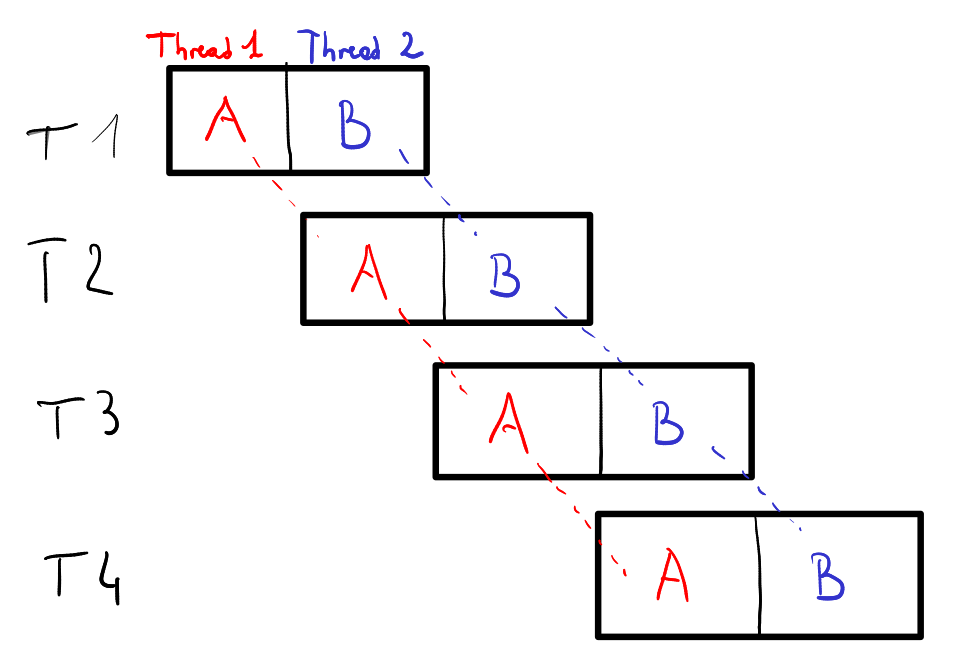
\includegraphics[scale=0.3]{prod_cons.png}
\end{center}
Tutte le parti A del task verranno eseguite dal thread 1 (\textbf{produttore}) e tutte le B dal 2 (\textbf{consumatore}). Di conseguenza se ogni parte richiede $1u$ di tempo, con questo schema serviranno $5u$.\\
Si rende necessario un modo di condividere le informazioni tra i due thread, ovvero condividere i risultati della parte A. Il secondo thread di contro deve rimanere in attesa finché non gli arrivano i risultati da poter elaborare nella parte B.\\
Per fare ciò si usano i \textbf{semafori}, in modo che il secondo thread rimanga in \textbf{wait} in attesa dei dati, e appena il primo ha finito di lavorare mette i dati nel buffer comune e fa una \textbf{post} che sblocca il secondo.\\
Questo meccanismo è utile anche considerando che non tutte le parti dei task siano effettivamente di durata uguale. In questa casistica quando il primo thread si porta avanti e arriva a calcolare il terzo task , deve mettersi in attesa per evitare di sovrascrivere il terzo risultato sopra al secondo che non è ancora stato elaborato.
\begin{center}
	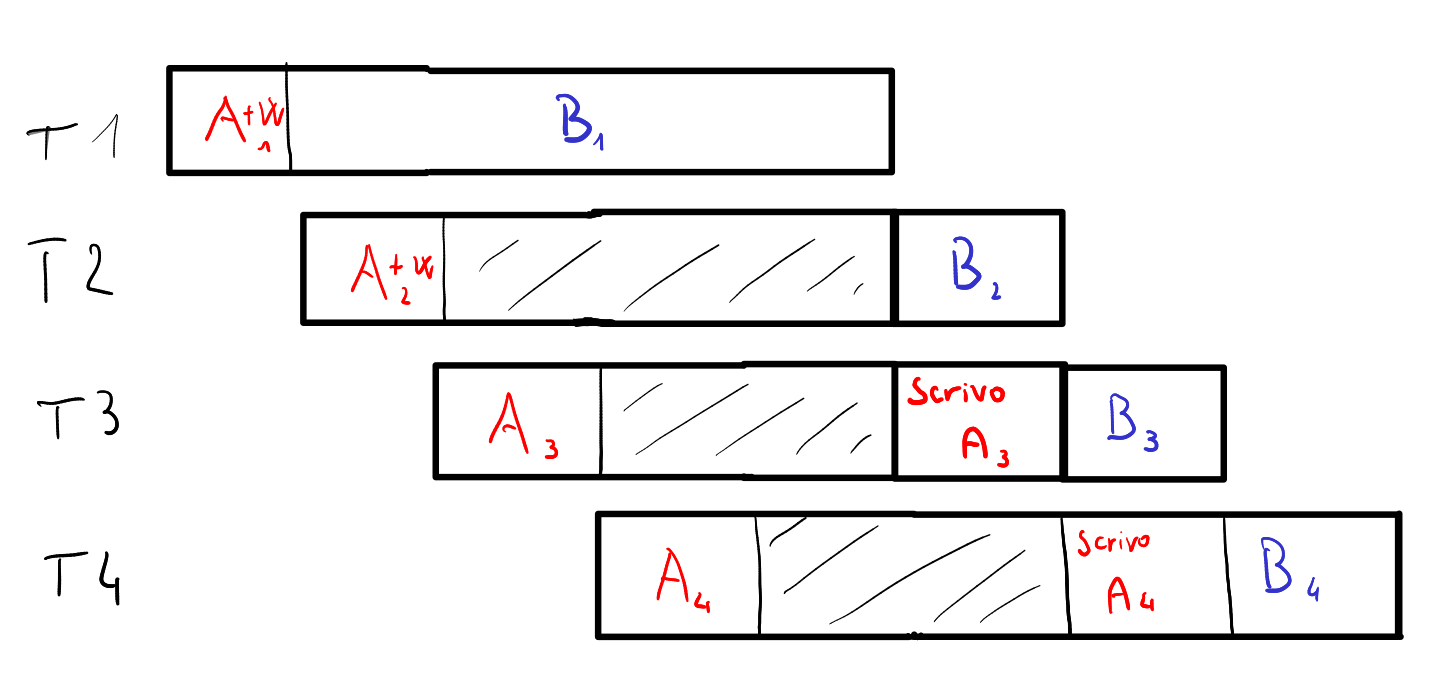
\includegraphics[scale=0.3]{prod_cons_2.png}
\end{center}
\begin{example}
	Esempio di esecuzione di 8 task con le varie fasi:
	\begin{table}[!h]
		\centering
		\begin{tabular}{|c|c|c|c|c|c|c|c|c|}
			\hline
			\textbf{\#Task} & \textbf{1} & \textbf{2} & \textbf{3} & \textbf{4} & \textbf{5} & \textbf{6} & \textbf{7} & \textbf{8} \\
			\hline
			Inizio calcolo & 0 & 2 & 3 & 4 & 5 & 6 & 7 & 8\\
			Tempo prod & 2 & 1 & 1 & 1 & 1 & 1 & 1 & 1 \\
			Fine calcolo prod & 2 & 3 & 4 & 5 & 6 & 7  &8  &9 \\
			Scrittura buffer & 2 & 3 & 4 & 5 & 6 & 7  &8  &9 \\
			Lettura cons & 2 & 3 & 4 & 5 & 6 & 7  &8  &9 \\
			Tempo cons& 1 & 1 & 1 & 1 & 1 & 1 & 1 & 1 \\
			Fine totale & 3 & 4 & 5 & 6 & 7  &8  &9 & 10 \\
			\hline
		\end{tabular}
	\end{table}
	Se cambiamo i tempi necessari al produttore e al consumatore:
	\label{example:prodcons}
	\begin{table}[!h]
		\centering
		\begin{tabular}{|c|c|c|c|c|c|c|c|c|}
			\hline
			\textbf{\#Task} & \textbf{1} & \textbf{2} & \textbf{3} & \textbf{4} & \textbf{5} & \textbf{6} & \textbf{7} & \textbf{8} \\
			\hline
			Inizio calcolo & 0 & 1 & 2 & 6 & 11 &16 & 21 & 26\\
			Tempo prod & 1 & 1 & 1 & 1 & 5 & 5 & 5 & 5 \\
			Fine calcolo prod & 1 & 2& 3 & 7 & 16 & 21  &26  &31 \\
			Scrittura buffer & 1 & 2 & 6 & 11 & 16 & 21  &26  &31 \\
			Lettura cons & 1 & 6 & 11 & 16 & 21 & 22  &26  &31 \\
			Tempo cons& 5 & 5 & 5 & 5 & 1 & 1 & 1 & 1 \\
			Fine totale & 6 & 11 & 16 & 21 & 22  &23  &27 & 32 \\
			\hline
		\end{tabular}
	\end{table}
	In questo caso abbiamo delle inefficienze in quanto produttore e consumatore devono aspettarsi a vicenda avendo tempistiche di lavoro diverse.
\end{example}
Per risolvere il problema descritto nell'esempio \ref{example:prodcons} è possibile aumentare la \textbf{grandezza del buffer}, permettendo di accumulare più di un singolo risultato della parte A alla volta e riducendo quindi i tempi.\\
Per implementare la soluzione usiamo due semafori:
\begin{itemize}
	\item \textbf{sem\_free\_slots}, inizializzato a $b$, indica il numero di slot dove il produttore può scrivere
	\item \textbf{sem\_data\_items}, inizializzato a $0$, indica il numero di oggetti scritti dal produttore che il consumatore deve elaborare
\end{itemize}
Se il produttore deve scrivere qualcosa effettua
\begin{lstlisting}[language=C]
	sem_wait(sem_free_slots);
\end{lstlisting}
e dopo aver aspettato effettua la scrittura del dato e poi
\begin{lstlisting}[language=C]
	sem_post(sem_data_items);
\end{lstlisting}
Quando invece il consumatore vuole un nuovo dato effettua
\begin{lstlisting}[language=C]
	sem_wait(sem_data_items);
\end{lstlisting}
che aspetta che ci sia un dato disponibile e mantiene aggiornato il numero di oggetti sul buffer. Legge poi il dato ed esegue
\begin{lstlisting}[language=C]
	sem_post(sem_free_slots);
\end{lstlisting}
che mantiene aggiornato il numero di slot liberi.\\
Dopo ogni operazione è mantenuto l'invariante:
\begin{equation*}
	sem\_free\_slots + sem\_data\_items = b
\end{equation*}
Per gestire le posizioni libere occupate nel buffer usiamo un indice $p$ per la prossima posizione dove scriverà il produttore e un indice $c$ per la prossima posizione dove legge il consumatore.\\
Grazie all'uso dei semafori abbiamo che:
\begin{equation*}
	c \leq p \leq c+b
\end{equation*}
Quando $c=p$, sem\_data\_items vale $0$ e $c$ non può avanzare oltre, quando invece $p=c+b$, sem\_free\_slots è $0$ e $p$ non può avanzare oltre. In questo modo facciamo finta di avere un buffer infinito ma accediamo alle posizioni $c\%b$ e $p\%b$ che sono tra $0$ e $b-1$.
\begin{example}
	Modifichiamo l'esempio \ref{example:threads_prime} implementando un buffer e dei semafori.
	\label{example:semafori}
	\begin{lstlisting}[language=C]
		#define Buf_size 10
		
		// Struct contenente i parametri di input e output di ogni thread 
		typedef struct {
			int quanti;   // output
			long somma;   // output
			int *buffer; 
			int *pcindex;
			sem_t *sem_free_slots;
			sem_t *sem_data_items;  
		} dati;
		
		// Funzione eseguita dai thread consumer
		void *tbody(void *arg)
		{  
			dati *a = (dati *)arg; 
			a->quanti = 0;
			a->somma = 0;
			int n;
			fprintf(stderr,"Consumatore %d partito\n",gettid());
			do {
				xsem_wait(a->sem_data_items,__LINE__,__FILE__);
				n = a->buffer[*(a->pcindex) % Buf_size];
				*(a->pcindex) +=1;
				xsem_post(a->sem_free_slots,__LINE__,__FILE__);
				if(n>0 && primo(n)) {
					a->quanti++;
					a->somma += n;
				}
			} while(n!= -1);
			fprintf(stderr,"Consumatore %d sta per terminare\n",gettid());
			pthread_exit(NULL); 
		}     
		
		int main(int argc, char *argv[])
		{
			// Leggi input
			if(argc!=2) {
				printf("Uso\n\t%s file\n", argv[0]);
				exit(1);
			}
			// Numero di thread ausiliari 
			int p = 1;
			assert(p>0);
			int tot_primi = 0;
			long tot_somma = 0;
			int e,n,cindex=0;    
			// Threads related
			int buffer[Buf_size];
			int pindex=0;
			// pthread_mutex_t mu = PTHREAD_MUTEX_INITIALIZER;
			pthread_t t[p];
			dati a[p];
			sem_t sem_free_slots, sem_data_items;
			xsem_init(&sem_free_slots,0,Buf_size,__LINE__,__FILE__);
			xsem_init(&sem_data_items,0,0,__LINE__,__FILE__);
			for(int i=0;i<p;i++) {
				// Faccio partire il thread i
				a[i].buffer = buffer;
				a[i].pcindex = &cindex;
				a[i].sem_data_items = &sem_data_items;
				a[i].sem_free_slots = &sem_free_slots;
				xpthread_create(&t[i],NULL,tbody,a+i,__LINE__,__FILE__);
			}
			fputs("Thread ausiliari creati\n",stderr);
			FILE *f = fopen(argv[1],"r");
			if(f==NULL) {perror("Errore apertura file"); return 1;}
			while(true) {
				e = fscanf(f,"%d", &n);
				if(e!=1) break; // Se il valore letto correttamente e==1
				assert(n>0);    // I valori del file devono essere positivi
				xsem_wait(&sem_free_slots,__LINE__,__FILE__);
				buffer[pindex++ % Buf_size]= n;
				xsem_post(&sem_data_items,__LINE__,__FILE__);
			}
			fputs("Dati del file scritti nel buffer\n",stderr);
			if(fclose(f)!=0) xtermina("Errore chiusura input file",__LINE__,__FILE__);
			// Terminazione threads
			for(int i=0;i<p;i++) {
				xsem_wait(&sem_free_slots,__LINE__,__FILE__);
				buffer[pindex++ % Buf_size]= -1;
				xsem_post(&sem_data_items,__LINE__,__FILE__);
			}
			fputs("Valori di terminazione scritti nel buffer\n",stderr);
			// Join dei thread e calcolo risultato
			for(int i=0;i<p;i++) {
				xpthread_join(t[i],NULL,__LINE__,__FILE__);
				tot_primi += a[i].quanti;
				tot_somma += a[i].somma;
			}
			xsem_destroy(&sem_data_items,__LINE__,__FILE__);
			xsem_destroy(&sem_free_slots,__LINE__,__FILE__);
			// pthread_mutex_destroy(&mu);
			printf("Trovati %d primi con somma %ld\n",tot_primi,tot_somma);
			return 0;
		}
	\end{lstlisting}
\end{example}
\begin{note}
	Come visto in \ref{note:mutex_efficiency} è importante dare il via libera agli altri thread tramite una \emph{post} del semaforo il prima possibile per garantire l'efficienza del codice.
\end{note}
Il problema di questo metodo è la \textbf{terminazione}. La strategia più semplice per segnalare al consumatore che il lavoro è finito è quello di passare un valore \emph{dummy} concordato in precedenza. Ad esempio nel caso \ref{example:semafori} abbiamo usato $-1$.

\begin{observation}
	Se invece di utilizzare un buffer di tipo circolare utilizzassi una pila, non sarebbe garantito l'ordine di elaborazione dei dati prodotti dei dati dal consumatore, che potrebbe trovarsi come primo dato il \emph{dummy} e terminare subito.
\end{observation}

\subsubsection{Condition variables}
Ci permette di utilizzare condizioni per fermare il thread personalizzate.
\begin{example}
	Supponiamo di avere diversi thread che eseguono diverse operazioni, ognuna con una necessità di memoria diversa. Il sistema ha a disposizione $100MB$ da dividere tra di loro. Si rende quindi necessario un controllore centrale che gestisca la cessione della memoria ai vari thread.\\
	Se ad esempio un primo thread richiede $20MB$, i disponibili diventano $80MB$. Quando poi un altro thread ne richiede ad esempio $90MB$, il controllore deve metterlo in attesa finché non ne sono disponibili di nuovo a sufficienza.
	\begin{lstlisting}
		fprintf(stderr,"%2d Assegnati: %3d. Rimanenti: %4d\n\n", gettid()%100,
		memoria_disponibile >= quante_ne_serve
	\end{lstlisting}
\end{example}
La comodità rispetto ai semafori è che in questi l'unico test possibile è verificare che il suo valore sia $\geq 0$ mentre in questo caso non siamo vincolati.\\
Una possibile implementazione è la seguente:
\begin{lstlisting}[language=C]
	// Struct che tiene traccia della memoria disponibile e 
	// contiene le variabili cond/mutex per regolarne l'utilizzo
	typedef struct {
		pthread_cond_t  *cv; // Condition variable
		pthread_mutex_t *mu; // Mutex
		int MB;       // Memoria attualmente disponibile
	} heap;
	
	// Simula allocazione con spazio limitato
	void richiedi(heap *h, int n) {
		// E' necessario che anche il ciclo while sia sotto lock del mutex
		xpthread_mutex_lock(h->mu,QUI);
		while(n>h->MB) {
			// In automatico viene rilasciato il mutex prima di addormentarsi
			xpthread_cond_wait(h->cv,h->mu,QUI);
			// Al risveglio del thread viene riacquisito il mutex (se ce ne sono diversi in attesa, il piu veloce lo prende, gli altri attendono)
		}
		h->MB -= n;
		xpthread_mutex_unlock(h->mu,QUI);
	}
	
	// Deallocazione
	void libera(heap *h, int n) {
		xpthread_mutex_lock(h->mu,QUI);
		h->MB += n;
		// Sveglia tutti i thread avvisando che ci sono risorse disponibili
		xpthread_cond_broadcast(h->cv,QUI);
		xpthread_mutex_unlock(h->mu,QUI); 
	}
	
	// Codice thread tipo 1, chiede 10,20,...,50
	void *tipo1(void *v) {
		heap *h = (heap *) v;
		for(int i=1;i<=5;i++) {
			int m = 10*i;
			richiedi(h,m);
			sleep(1);
			libera(h,m);
		}
		return NULL;
	}
	
	// Codice thread tipo 2, chiede 15,25,...,55
	void *tipo2(void *v) {
		heap *h = (heap *) v;
		for(int i=1;i<=5;i++) {
			int m = 10*i+5;
			richiedi(h,m);
			sleep(1);
			libera(h,m);
		}
		return NULL;
	}
	
	int main(int argc, char *argv[])
	{		
		// Inizializza heap 
		pthread_cond_t c = PTHREAD_COND_INITIALIZER;
		pthread_mutex_t m = PTHREAD_MUTEX_INITIALIZER;
		heap h;
		h.cv = &c; h.mu = &m;
		h.MB = mem;
		
		// Esegue i thread
		pthread_t t[nt];
		// Esegue un thread tipo1
		xpthread_create(&t[0],NULL,&tipo1,&h,QUI);
		for(int i=1;i<nt;i++)
		// Esegue nt-1 thread di tipo 2
			xpthread_create(&t[i],NULL,&tipo2,&h,QUI);
		
		// Attende terminazione thread e termina
		for(int i=0;i<nt;i++)
			xpthread_join(t[i],NULL,QUI);
		xpthread_cond_destroy(&c,QUI);
		xpthread_mutex_destroy(&m,QUI);
		
		return 0;
	}
\end{lstlisting}

\begin{example}
	Un esempio di implementazione di una soluzione al problema dei \textbf{produttori e consumatori} usando le variabili condivise è la seguente:
	\begin{lstlisting}[language=C]
		typedef struct {
			int readers;
			bool writing;
			pthread_cond_t cond;   // Condition variable
			pthread_mutex_t mutex; // Mutex associato alla condition variable
		} rw;
		
		// Inizializza rw, ne scrittori ne lettori 
		void rw_init(rw *z)
		{
			z->readers = 0;
			z->writing = false;
			xpthread_cond_init(&z->cond,NULL,QUI);
			xpthread_mutex_init(&z->mutex,NULL,QUI);
		}
		
		// Inizio uso da parte di un reader
		void read_lock(rw *z)
		{
			pthread_mutex_lock(&z->mutex);
			while(z->writing==true)
			pthread_cond_wait(&z->cond, &z->mutex);   // attende fine scrittura
			z->readers++;
			pthread_mutex_unlock(&z->mutex);
		}
		
		// Fine uso da parte di un reader
		void read_unlock(rw *z)
		{
			assert(z->readers>0);  // Ci deve essere almeno un reader (me stesso)
			assert(!z->writing);   // Non ci devono essere writer 
			pthread_mutex_lock(&z->mutex);
			z->readers--;                  // Cambio di stato       
			if(z->readers==0) 
			// A differenza della broadcast, la signal sveglia solamente uno dei thread in attesa
			pthread_cond_signal(&z->cond); 
			pthread_mutex_unlock(&z->mutex);
		}
		
		// Inizio uso da parte di writer  
		void write_lock(rw *z)
		{
			pthread_mutex_lock(&z->mutex);
			while(z->writing || z->readers>0)
			// Attende fine scrittura o lettura
			pthread_cond_wait(&z->cond, &z->mutex);   
			z->writing = true;
			pthread_mutex_unlock(&z->mutex);
		}
		
		// Fine uso da parte di un writer
		void write_unlock(rw *z)
		{
			assert(z->writing);
			pthread_mutex_lock(&z->mutex);
			z->writing=false;               // Cambio stato
			// Segnala a tutti quelli in attesa 
			pthread_cond_broadcast(&z->cond);  
			pthread_mutex_unlock(&z->mutex);
		}
	\end{lstlisting}
\end{example}
\end{document}
